\section{Introduction}

The \texttt{optimize} method is called and within it a new \texttt{ClassGen} object is created. Then the \texttt{ConstantPool} and the unoptimized methods are retrieved from the \texttt{ClassGen} object. Then, \texttt{optimize} iterates over these methods and calls \texttt{performFolding} for each one. Once there are no more methods remaining, the optimized code is generated. The general process of this optimisation is depicted in figure \ref{fig:overview}.

\begin{figure}[h]
\centering
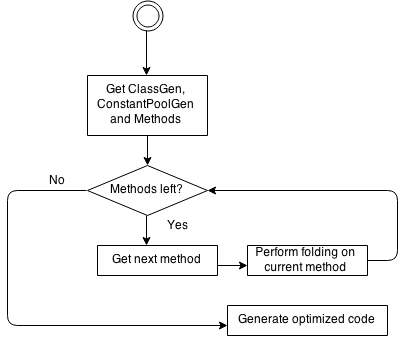
\includegraphics[scale=0.6]{figures/overview}
\caption{The general process of optimisation}
\label{fig:overview}
\end{figure}

In the following section \ref{sec:classification}, we will provide further explanation on how we classified the different bytecode instruction types. It is followed by a detailed description of out most important functions (section \ref{sec:description}). Since every in section \ref{sec:classification} described instruction type is handled differently, every particular explanation is supported by an appropriate flow chart diagram. The report closes with an example showing the difference between unoptimized and unoptimized code (section \ref{sec:example}).